\input ../hdr.tex

\section{Mantle transport}

\subsection{Phase behavior}

Three phases in total with 2 solid phases:

\begin{itemize}
		  \item Phase 1 can melt into fluid. 
		  \item Phase 2 can also melt into fluid.
		  \item Different substances in fluid can react with
each other.
\end{itemize}

\begin{center}
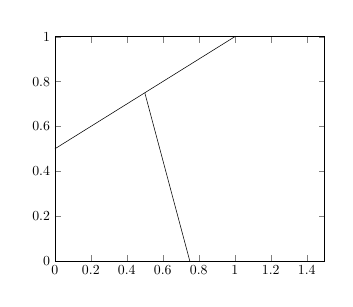
\begin{tikzpicture}[scale=0.5]
		  \begin{axis}[xmin=0,ymin=0,xmax=1.5,ymax=1]
					 \addplot[smooth, color=black] coordinates {(0,0.5) (1,1)};
					 \addplot[smooth, color=black] coordinates {(0.5,0.75) (0.75,0)};
		  \end{axis}
\end{tikzpicture}
\end{center}

Set up equations for component 1,
which exhausts phase 1.
Similarly, phase 2 is all component 2.
Denote $c_{i,j}$ as component i in phase j.\\

Thus, the following equations can be derived:\\

Phase 1:
\begin{equation}
		  c_{1,1} = \rho_1 = \frac{M_{1,1}}{V_1} \hspace{0.5cm}c_{2,1} = 0 = M_{2,1} 
\end{equation}

\indent \indent Note: $\rho_1 = \rho_1(p_1)$ only.\\

Phase 2:
\begin{equation}
		  c_{1,2} = 0 = M_{1,2} \hspace{0.5cm}c_{2,2} = \rho_2 = \frac{M_{2,2}}{V_2}
\end{equation}

\indent \indent Note: $\rho_2 = \rho_2(p_2)$ only.\\

Phase fluid:

\begin{equation}
		  c_f = c_{1,f} = \frac{M_{1,f}}{V_f}, \hspace{0.5cm}, c_{2,f} = \frac{M_{2,f}}{V_f}
\end{equation}

Additional relations and negligible diffusion:

\begin{equation}
		  \phi_f V_f \sim (\phi_1 + \phi_2)V_s, \hspace{0.5cm} \phi_f D \nabla c_f \sim 0
\end{equation}

\vspace{0.5cm}

Transport variable $\bar{c}$ is defined as following:

\begin{equation}
		  \begin{aligned}
					 \overline{c} &= \phi_f c_{1,f} + \phi_1 c_{1,1} + \phi_2 c_{1,2}\\
					 &= \phi_fc_f + \phi_1c_s
		  \end{aligned}
\end{equation}

Note

\begin{equation}
					 \phi_f = \frac{V_f}{V}, \hspace{0,5cm}, \phi_1 = \frac{V_1}{V}, \hspace{0.5cm}, \phi_2 = \frac{V_2}{V}
\end{equation}

\begin{equation}
\phi_s = \phi_1 + \phi_2
\end{equation}

\begin{equation}
\phi_f + \phi_1 + \phi_2 = \phi_f + \phi_s = 1
\end{equation}

Then

\begin{equation}
		  \begin{aligned}
					 \overline{c} = \phi_f c_f + \phi_1 c_s &= \frac{V_f}{V}\frac{M_{1,f}}{V_f} + \frac{V_1}{V}\frac{M_{1,1}}{V_1}\\
					 &=(M_{1,f} + M_{1,1})/V\\
					 &=M_1/V
		  \end{aligned}
\end{equation}

The transport equation is now converted into:

\begin{equation}
		  \overline{c}_t + \nabla \cdot (\overline{cv} - \phi_f D \nabla c_f)=0
\end{equation}

Two possible approaches:\\

(1) Linearize phase behavior:
\begin{equation}
		  \phi_f c_f = \kappa(\overline{H}, \overline{c}) \overline{c} \approx \kappa \overline{c}
\end{equation}

(2) Operator split by phase:
\begin{equation}
		  \left \{
		  \begin{aligned}
					 (\phi_f c_f)_t + \nabla \cdot (\phi_f c_f v_f - \phi_f D \nabla c_f) &= \Gamma \approx 0 \\
					 (\phi_1 c_s)_t + \nabla \cdot (\phi_1 c_s v_s) &= -\Gamma \approx 0
		  \end{aligned}
		  \right .
\end{equation}

\indent \indent Flash calculation to approx $\Gamma$.\\

We pursue first approach (Eqn. 11). Note:

\begin{equation}
0 \leq \kappa \leq 1
\end{equation}

Since,

\begin{equation*}
		  \phi_f c_f = \kappa \overline{c} = \kappa(\phi_f c_f + \phi_1 c_s)
\end{equation*}

moreover,

\begin{equation*}
		  \overline{c} = \phi_f c_f + \phi_1 c_s
\end{equation*}

$\Rightarrow$

\begin{equation}
		  \phi_1 c_s = \overline{c} - \phi_f c_f = (1-\kappa) \overline{c}
\end{equation}

now we have

\begin{equation*}
		  \begin{aligned}
					 \overline{cv} &= \phi_f c_f v_f + \phi_1 c_s v_s + \phi_2 \cdot 0 v_s\\
					 &= (\kappa v_f + (1-\kappa)v_s)\overline{c}
\end{aligned}
\end{equation*}

$\Rightarrow$

\begin{equation}
		  \overline{cv} = v_e \overline{c}
\end{equation}

\begin{equation}
		  v_e = Kv_f + (1-K)v_s
\end{equation}

So previous equation becames:

\begin{equation}
		  \overline{c}_t + \nabla \cdot (v_e \overline{c} - \phi_f D \nabla c_f) = 0
\end{equation}

Also

\begin{equation}
		  \begin{aligned}
		  \phi_f D \nabla c_f &= \phi_f D \nabla (\frac{\kappa \overline{c}}{\phi_f})\\
		  &= \kappa D \nabla \overline{c} + \overline{c}D(\nabla \kappa - \kappa \nabla ln(\phi))
		  \end{aligned}
\end{equation}

Thus transport equation (17) becomes:

\begin{equation}
		  \overline{c}_t + \nabla \cdot (v_e^* \overline{c} - \kappa D \nabla \overline{c}) = 0
\end{equation}

where

\begin{equation}
		  \begin{aligned}
					 v_e^* &= v_e - D (\nabla K - K \nabla ln(\phi))\\
					 &= \kappa v_f + (1-K)v_s - D(\nabla \kappa - \kappa \nabla ln(\phi))
		  \end{aligned}
\end{equation}

Then phase calculation for new $c_f$, $c_s$, $\phi_f$, $\phi_1$.\\

Questions:

\begin{itemize}
		  \item 1. Is approach (11) better than (12)?
		  \item 2. Can we approximate the nonlinearity in $\kappa(\bar{c})$ to solve (19) more accurately?
		  \item 3. Can we get $\kappa(\bar{c})$ itself? Then solve (19) without needing flash calculatio.
\end{itemize}

\newpage

\subsection{Thermodynamics}

\indent \indent Let

\begin{equation}
		  E = \overline{\rho e} = \text{internal energy/volume}
\end{equation}

Thus the energy conservation equation is defined as:

\begin{equation}
		  \frac{\partial}{\partial t} \overline{\rho e} + \nabla \cdot (\overline{\rho e v} - \overline{K} \nabla T) = 0
\end{equation}

Now suppose that 

\begin{equation}
		  \begin{aligned}
					 \phi_{f}\rho_{f}e_{f} &= \lambda(\overline{H},\overline{C})\overline{\rho e} = \lambda \overline{\rho e} = \lambda E\\
					 &= \lambda (\phi_f \rho_f e_f + \phi_1 \rho_1 e_1 + \phi_2 \rho_2 e_2)
		  \end{aligned}
\end{equation}

where

\begin{equation}
		  \phi_1 \rho_1 e_1 + \phi_2 \rho_2 e_2 = (1-\lambda)\overline{\rho e}
\end{equation} Thus the resulting energy conservation law is: \begin{equation} E_t + \nabla \cdot (v_e^E E - \overline{K}\nabla T) = 0 \end{equation} which is derived similarly with what we have done above.  where average velocity is defined as: \begin{equation} v_e^E = \lambda v_f + (1-\lambda) v_s \end{equation}

Now

\begin{equation}
\overline{K} = \phi_f K_f + \phi_1 K_1 + \phi_2 K_2
\end{equation}

where

\begin{equation}
		  \nabla T(C,E) = \frac{\partial T}{\partial C}\nabla C + \frac{\partial T}{\partial E}\nabla E
\end{equation}

At each time step, temperature distribution will be 
obtained directly from Marc's code, as well as
the corresponding spactial gradient of temperature.
The convergence of this method will be researched.

\newpage

\subsection{Darcy-Stokes system}

Quotes: The model transitions dynamically in time from a nonporous single phase Stokes to a 
two-phase porous medium. 
The Darcy part will mathematically degenerate in regions where the porosity is zero.

The  resulting stokes system is described as following:

		  \begin{equation*}
					 \left \{
					 \begin{aligned}
								\boldsymbol u + \frac{k_0 \phi^{2+2\Theta}}{\mu_f}\nabla q_f &= 0\\
								\mu_s \nabla \cdot \boldsymbol u + \frac{\phi}{1-\phi}(q_f-q) &=0 \\
								\nabla q - \nabla \cdot \hat{\boldsymbol \sigma}(\boldsymbol v_s) &= -(1-\phi)\rho_r \boldsymbol g\\
								\mu_s \nabla \cdot \boldsymbol v_s - \frac{\phi}{1-\phi}(q_f-1) &=0
					 \end{aligned}
					 \right .
		  \end{equation*}

where pressure potentials are defined as:

		  \begin{equation*}
            \begin{aligned}
						  q_f &= p_f - \rho_f g z \\
						  q_s &= p_s - \rho_f g z
				\end{aligned}
		  \end{equation*}

and the mixture potential is therefore:

\begin{equation*}
		  p_f - p_s = q_f - q_s = \frac{1}{1-\phi}(q_f - q)
\end{equation*}

the compatibility condition is given as:

\begin{equation*}
		  \int_{\partial \Omega}(g_r + \boldsymbol g_s \cdot \nu)ds = 0
\end{equation*}

The scaled formulation is also defined:

\begin{equation*}
		  \begin{aligned}
					 \tilde{\boldsymbol v}_r &= \phi^{-1-\Theta} \boldsymbol u\\
					 \tilde{q}_f = \phi^{1/2}q_f
		  \end{aligned}
\end{equation*}

Then the problem is reformulated as :

\begin{equation*}
					 \left \{
					 \begin{aligned}
								\tilde{\boldsymbol v}_r + \frac{k_0 \phi^{1+\Theta}}{\mu_f}\nabla (\phi^{1/2} q_f) &= 0\\
								\mu_s \phi^{-1/2} \nabla \cdot (\phi^{1+\Theta}\tilde{\boldsymbol v}_r) + \frac{1}{1-\phi}(\tilde{q}_f-\phi^{1/2}q) &=0 \\
								\nabla q - \nabla \cdot \hat{\boldsymbol \sigma}(\boldsymbol v_s) &= -(1-\phi)\rho_r \boldsymbol g\\
								\mu_s \nabla \cdot \boldsymbol v_s - \frac{\phi^{1/2}}{1-\phi}(\tilde{q}_f-\phi^{1/2}q) &=0
					 \end{aligned}
					 \right .
\end{equation*}

Implmentation of the methods on rectangular meshes:

\begin{equation*}
\begin{pmatrix}
		  A & -B_\phi & 0 & 0 \\
		  B^T_\phi & C_{f,\phi} & 0 & -C_{f,s,\phi} \\
		  0 & 0 & D_\phi & -B \\
		  0 & -C^T_{f,s,\phi} & B^T & C_{s,\phi}
\end{pmatrix}  \begin{pmatrix}
		  \tilde{v}_r \\
		  \tilde{q}_f \\
		  v_s \\
		  q
\end{pmatrix} = \begin{pmatrix}
		  \alpha _\phi\\
		  0 \\
		  b_\phi\\
		  0
\end{pmatrix}
\end{equation*}

Using Schur complement, the remaining Stokes-like systme with two pressure potentials 
are solved as:

\begin{equation*}
		  \begin{pmatrix}
					 B^TA^{-1}B_{\phi} + C_{f,s,\phi} & -C_{f,s,\phi}\\
					 -C_{f,s,\phi} & B^TD^{-1}B_{\phi} + C_{f,s,\phi}
		  \end{pmatrix} \begin{pmatrix}
        \tilde{q}_f \\
					 q
		  \end{pmatrix} = \begin{pmatrix}
         -B^T_{\phi}A^{-1} \alpha_\phi \\
					 -B^TD^{-1}_\phi b_\phi
		  \end{pmatrix}
\end{equation*}

\newpage

\subsection{Coupled Darcy-Stokes, transport and thermal system}

The following coupled systems will be dealt with:\\

Darcy-Stokes system:

\begin{equation*}
					 \left \{
					 \begin{aligned}
								\tilde{\boldsymbol v}_r + \frac{k_0 \phi^{1+\Theta}}{\mu_f}\nabla (\phi^{1/2} q_f) &= 0\\
								\mu_s \phi^{-1/2} \nabla \cdot (\phi^{1+\Theta}\tilde{\boldsymbol v}_r) + \frac{1}{1-\phi}(\tilde{q}_f-\phi^{1/2}q) &=0 \\
								\nabla q - \nabla \cdot \hat{\boldsymbol \sigma}(\boldsymbol v_s) &= -(1-\phi)\rho_r \boldsymbol g\\
								\mu_s \nabla \cdot \boldsymbol v_s - \frac{\phi^{1/2}}{1-\phi}(\tilde{q}_f-\phi^{1/2}q) &=0
					 \end{aligned}
					 \right .
\end{equation*}

Transport and thermal system:

\begin{equation*}
		  \left \{
					 \begin{aligned}
								\overline{c}_t + \nabla \cdot (v_e^* \overline{c} - \kappa D \nabla \overline{c}) &= 0\\
								E_t + \nabla \cdot (v_e^E E - \overline{K}\nabla T) &= 0
					 \end{aligned}
					 \right .
\end{equation*}

\newpage

\subsection{Spatial and time discretization}

The general procedure of solving coupled stokes and transport system 
will be shown as follows:

\tikzstyle{block} = [rectangle, draw, fill=blue!20,
text width=5em, text centered, rounded corners, minimum height=4em]
\tikzstyle{line} = [draw]

\begin{tikzpicture}[align=center, node distance=4cm,auto]
		  % Place nodes
		  \node[block] (stokes) {Darcy-Stokes system};
		  \node[block] (transport) {Transport diffusion problem};
        \node[block] (energy) {Thermal problem};
		  % Draw edges
        \path[line] (stokes) -- (transport);
		  \path[line] (transport) -- (energy);
\end{tikzpicture}


\end{document}
